\chapter{Analysis}
\label{analysis}

\lettrine[lraise=0.1, nindent=0em, slope=-.5em]{\color{Violet}T}{his} chapter contains analytical part of the thesis, beginning with requirements analysis of the current situation, followed by analysis of the problems. Next, a requirement list for the new e-learning course  is compiled, followed by choosing methodology for development of the e-learning course. 

\section{Problem Analysis}
\label{Problem Analysis}


Lack of skilled \gls{ICT} specialist is a well-known problem in Estonia \citep{website:ict_puudu, website:ict_needs}. However, several higher education institutions have increased the number of spots in \gls{ICT} in their curricula, the number of graduated students is still insufficient for the field requirements~\citep{website:TU_ict,website:itc_facts}. Moreover,  continuous changing of the field calls for continuous development of curricula. Also continuous learning is common in \gls{ICT} field because its changing. Therefore, modernisation of the  \gls{ICT} curriculum and offering continuous education courses are priority for \gls{EITC} to maintain professionalism of graduated specialists.

In order to facilitate a curriculum development process \gls{EISA} contacted \gls{EITC} presenting a problem: Lack of skilled and security-aware system administrators. Then, an initial proposal for solution to deal with the problem is provided as seen in Appendix~\ref{Letter from CERT.EE to the Rector of Estonian IT College} on page ~\pageref{Letter from CERT.EE to the Rector of Estonian IT College}. However, instead of accepting the solution without questioning the curriculum heads of \gls{EITC} arranged several workshops for initial investigation of the problem and divided it to separate sub-problems and areas. For ensuring wider view of the problem, several experts from private companies, telecoms, banks, small business and start-ups were involved. Author of this thesis characterized the proposal and established and negotiated the requirements for changes and composed an action plan.

During curricula development workshops, the author described the main reasons of the problem as following:

First, many system administrators acquired their knowledge through self-education. However, continuous study is common in \gls{ICT} field as the level of the specialists is varying and they do not have sufficient knowledge to build secure infrastructure.

Second, the applied education field does not provide qualification needed for managing secure infrastructure services. Therefore changes to curriculum are needed to fill the cap.

Third, it is usual in continuous education field that private companies offer several courses on configuring and securing infrastructure, networks and services. However, those trainings are usually vendor-based and heavily focused on promoting proprietary technologies without emphasising broader knowledge in security field.

Fourth, the system administrators in local government or municipal field have heterogeneous level of skills and knowledge. Therefore, supporting and helping them is quite problematic for \gls{CERT.EE}.

Fifth, all courses (yet to be developed) should be associated with practical applicability of the theoretical knowledge and should contain largely practical hands-on classes. Moreover, all materials should be based on non-proprietary technology, such as \gls{OpenBSD} or \gls{GNU/Linux}.

Sixth, the study program should focus on practical learning-by-doing approach to \gls{ICT} subjects.
 Moreover, using virtual and game-like environments is a contemporary approach for teaching IT System administration and programming focused on the cyber security requirements increases student motivation. Today the studies are too focused on the lecture form, practical classes are too simple and fail to reflect the real situation.

 
In conclusion, the security field in \gls{EITC} should be implemented by modifying existing courses and developing new subjects. Therefore, the author redesigns the IT system administration curricula in \gls{EITC} to mitigate the problems.



\section{Related Work}
\label{Related Work}
Designing an e-course is a challenge that has been met by many lecturers and instructional developers. Moreover, the popularity of the cyber security related subjects in information and communications technology ICT curricula is growing and become a "student’s magnet" for higher educational institutes \citep{CyberIsHot}. Thus it is possible to gain additional information by analysing related curricula and cyber security exercises  in several higher educational institutions and analysing instructional design methodologies to achieve goals of this thesis. Moreover, when designing a practical course it is also important to investigate courses in the given region and in the world. However, as it is not possible to investigate a large number of courses and resources, it is the author’s opinion that by reviewing several well-known courses, trainings, challenges and articles the amount of gathered information is sufficient in minimal level for developing an e-learning course.


\subsection{Cyber defence courses in Universities and Cyber exercisers}
Cyber defence exercisers can be categorized as practical exams and  expected skillsets of those events  can provide valuable information for curricula/course development process.

One comprehensive paper, "Collective Views of the NSA/CSS Cyber Defense Exercise
on Curricula and Learning Objectives" about National Security describes how the National Security
Agency/Central Security Service (NSA/CSS) annual Cyber Defense Exercise (\gls{CDX}) influences curricula and studies at eight US federal service academies \citep{adams_CDX_curricula}. For example, the student members of the Association for Computing Machinery (ACM) can participate in \gls{CTF} exercisers and  visit several security conferences \citep{adams_CDX_curricula}.

In University of Tartu several courses include relevant topics. For example, Computer Security course  contains also 14 practical classes \footnote{Computer Security course   \url{https://courses.cs.ut.ee/2012/turve/fall/Main/HomePage} (2013-05-21)}, System Administration course  provides a good starting point for GNU/Linux and basic system administration \footnote{ System Administration course  \url{https://courses.cs.ut.ee/2013/syshald/spring/Main/Loengud} (2013-05-21)}
University of Tartu offers more security related courses but for this particular thesis those two are most important because they are practical and related to system administrators field.

In Tallinn University of Technology (\gls{TUT}) several relevant courses are held as: Information Systems Hacking Attacks and Defence, Simulation of Attacks and Defense, Log Mining and Disk Forensics \footnote{wiki - lambda.ee \url{http://lambda.ee/wiki/Cyber_security_2012_second_year} (2013-05-21)}

Those courses are designed to give good hands-on experience on the field, in the author’s opinion, these are the best courses available in the region. However, in \gls{EITC} all this material can not be covered due curricula limitations but knowledge gathered on those courses will help to develop this particular e-learning course.

\subsection{Courses in private companies and other organizations}

Two days course "Hands-on Hacking Essentials" given by Clarified Security OÜ contains Reconnaissance and information gathering, Privilege escalation, Jumping the (fire)wall, BackTrack 5, Remote exploitation, Attack Tool-sets \citep{website:clarifiedsecurity_hohe}. Therefore, the given introduction should be a standard part of applied \gls{ICT} curricula. However, the course is too expensive to be integrated it into \gls{EITC} curricula. Another course offered by Clarified Security OÜ is the "Web Application security essentials" with duration of four days, focuses on to client side attacks and server side attacks and provides a systematic and well covered overview of the field \citep{website:clarifiedsecurity_hohe}.

However, both courses are designed  keeping offensive aspects in mind and their basics should also be covered in \gls{EITC} curricula because defending a system also requires basic offensive knowledge and skills.


The SANS Institute organizes extensive security trainings also in online form \citep{website:SANS}. Moreover, the institute shares free online resources for security topics \footnote{SANS - Reading Room \url{https://www.sans.org/reading_room/} (2013-05-21)} When developing a curriculum, the topics and best practices from SANS Institute should be worked through for to clarify learning outcomes and tools what can be used.

Last but not least, the \gls{OWASP} project provides good and reusable study materials  for theoretical and as well a practical guides as \gls{OWASP} Application Security Verification Standard (\gls{ASVS}) Project \footnote{\gls{OWASP}  (\gls{ASVS}) Project \url{https://www.owasp.org/index.php/Category:OWASP_Application_Security_Verification_Standard_Project} (2013-05-21)} .

\subsection{Large scale cyber security exercisers}
Several Cyber Defense Exercises (\gls{CDX}) are focused to training defence teams called Blue Teams \citep{website:NATO_CCD_COE,schepens_CDX}. It has been argued that \gls{CDX} is should be a part of  any computer security curricula in addition to the classroom learning \citep{adams_CDX_curricula}. International Cyber Defence Exercise Locked Shields is a defence exercise organised by NATO Cooperative Cyber Defence Centre of Excellence (\gls{NATO CCD COE}) and partners  \citep{website:NATO_CCD_COE}. 

The Blue Teams were the main training audience.
Skillset expected from the blue team technicians in International Cyber Defence Exercise Locked Shields 2012 according to action report was the following \citep{website:NATO_CCD_COE}:
\begin{itemize}
\item Administration of Windows domain, Active Directory, Windows workstation
\item Administration of Linux servers such as Debian and Ubuntu distributions
\item Firewalling (Netfilter based)
\item Knowledge about common network protocols/services and technologies as \gls{DNS}, \gls{NTP}, \gls{DHCP}, \gls{HTTP}, \gls{HTTPS}, \gls{SMTP}, \gls{POP3}, \gls{IMAP}, \gls{SSH}, \gls{FTP}, \gls{RADIUS}
\item \gls{KVM} virtualization platform
\item Web application technologies (\gls{HTML}, client-side and server-side scripting
such as JavaScript and \gls{PHP}, \gls{SQL} databases such as \gls{MySQL})
\item Administering of network devices (CISCO IOS, routing protocols)
\item Scripting skills in Perl
\end{itemize}

For large scale \gls{CDX} events the stability of the environment is always an issue \citep{website:NATO_CCD_COE,schepens_CDX}. {\color{red} Therefore, monitoring and IT service help are also fields that need investigation for environments where all students can start theirs virtual labs. }

\section{Choosing Methodology for Developing an e-course}

Developing an e-course can be done without using design methodology but systematic approach should give more effective results. In principle, a common systematic method to develop an (e-learning) course is applying the Instructional System Design \gls{ISD} (sometimes cited as  Instructional Design \gls{ID}) model \citep{website:id_models}. However, several \gls{ISD} models exist and can be divided into three classes: behaviorism, cognitivist and prescriptive design \citep{website:id_models}. This thesis uses Prescriptive Design Model, more specifically the \gls{ADDIE} process because the method is used in Estonia and recommended for designing e-learning course \citep[p.~5]{OppeArenduskeskus2010}. Moreover, the \gls{ADDIE} model is not only a widespread model that can be customized to meet specific needs, but it is a commonly used effective model for instructional  design \citep{ieee_addie_1607206}.

The methodology used to develop this e-course should encourage student activity in learning process. Moreover, student should have possibility to choose learning speed, place and time. Today's students have different learning styles and background and methodology should should take individual differences into consideration.

Developed e-course should support people with disabilities. In \gls{EITC} several people have hearing impairment and all important materials should also be presented without audio. For example, in screen-casts videos all important information should also be written on screen or added as transcript.

Today’s learning environment should support student communities where students can act as mentors and also feel part of the study program. Course integration with student driven initiative like forums, blogs, wiki pages and other collaborative learning methods should be encouraged and not restricted.

 However, the \gls{ADDIE} model has several weaknesses such as being too waterfall type model because it is not iterative \citep{website:weakesses_of_ADDIE_model}. Alternatively The Dick and Carey Model is used to design instructions \citep{dick2005systematic}. However, the Estonian best practice guide to designing a high-quality e-learning course is based on \gls{ADDIE} model \citep{OppeArenduskeskus2010}. Although the \gls{ADDIE} model is not modelling anything and technically it should be called a \gls{ISD} framework \citep{bichelmeyer2004addie}, in this thesis the term \gls{ADDIE} model is used because this name is commonly known and used for designing e-learning courses \citep{bichelmeyer2004addie, OppeArenduskeskus2010}.
In conclusion, the \gls{ADDIE} model was chosen to develop a particular cyber security e-learning course and the model itself is described in the following section.

\subsection{The ADDIE Model}

The \gls{ADDIE} model is used for creating different types of instructions such as courses, trainings \citep{website:addie, lohr1998using}. Moreover, the ADDIE method is  used to provide a systematic, iterative course development process with feedback-based approach to improve quality of study \citep{website:using_addie}.

The ADDIE model contains five stages: Analysis, Design, Development, Implementation and Evaluation as seen in Figure~\ref{figure:the addie model} \citep{website:addie}.


\begin{figure}[H]
 \centering 
 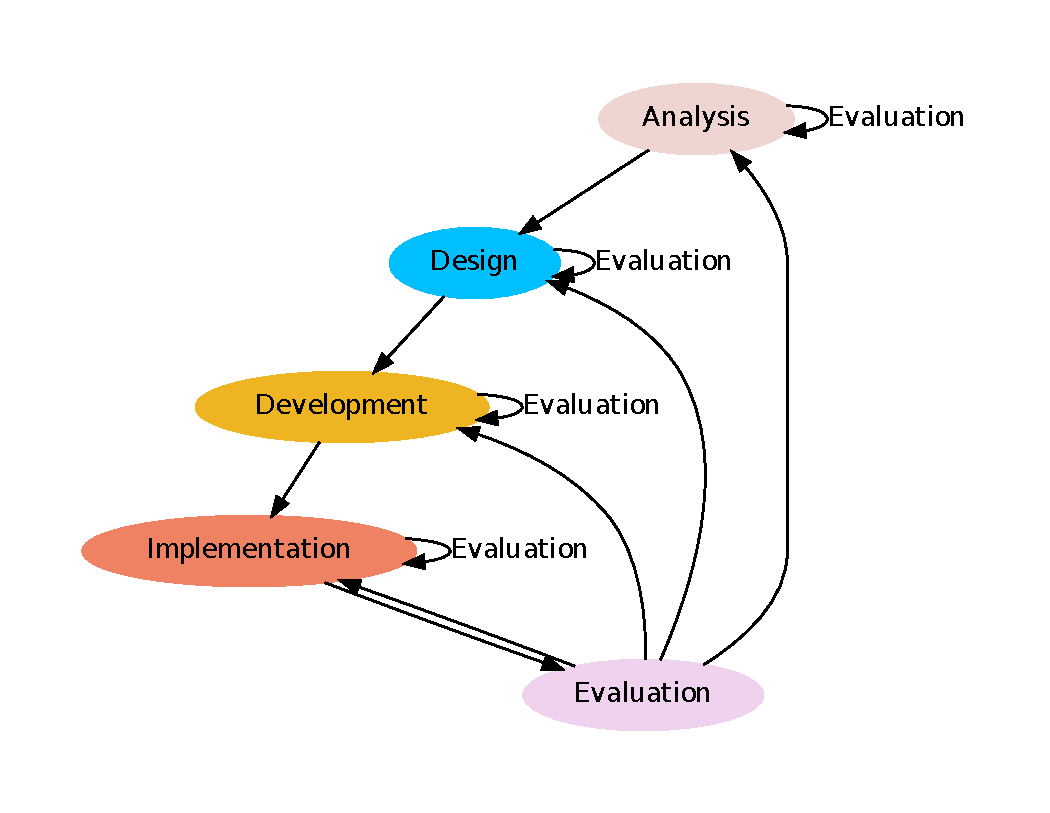
\includegraphics[width=0.6\textwidth]{addie_model.pdf}
 \rule{35em}{0.5pt} 
 \caption{The ADDIE model} 
 \label{figure:the addie model} 
\end{figure}

Firstly, the goal of the analysis phase is exploring of the gap between goal and existing situation. Therefore, instructional goals, current situation, learner, objectives are investigated in this phase~\citep{chen2007learning, website:addie}.

Secondly, the design phase focuses on the following areas: assessments design, learning content, learning strategies and course format \citep{chen2007learning, website:addie}.


Thirdly, the work of development includes creating the course materials, choosing methodology and technologies, testing material using run-through with a small group. \citep{OppeArenduskeskus2010, website:addie, chen2007learning}.


Fourthly, the implementation stage describes implementing the above work of three previous steps and gives possibility to evaluate full course in evaluation phase \citep{chen2007learning, website:addie}.


Finally, the evaluation phase is for assessing the learning effect through evaluation. Although, the evaluation process takes place in every stage as seen in Figure~\ref{figure:the addie model} the final evaluation focuses on the whole course and the feedback from students and lecturers, output of this phase is valuable for next courses \citep{OppeArenduskeskus2010, website:addie}.

\section{Analysis of the e-learning course}
According to the \gls{ADDIE} model, the analysis stage establishes goals of the course and evaluation of the current situation and strategy for implementing goals followed by analysis of the learners and the content of the course \citep{website:addie}.

The analysis phase of the \gls{ADDIE} model contains four sub-phases \citep{website:addie}.
\begin{enumerate}
\item Instructional Goals -- main objective plan for new course;
\item Instructional Analysis -- analysis of the current situation;
\item Learner Analysis -- target group properties such as previous knowledge about the field;
\item Learning Outcomes -- list of knowledge and skills to achieve instructional goals.
\end{enumerate}


\subsection{Instructional Goals}
The Instructional Goals and learning objectives should be established before designing new course as they provide answers to the student’s questions: Why should I study this topic, what will I learn during the course and how will I be evaluated? \citep{website:addie}.


The instructional goals of the new course were established by using interviews with \gls{EISA} and several companies. Therefore, the technologies system administrators need to know were listed.  Moreover, additional input to establish goals derives from analysis of the current curriculum.

The list of discussed topics is too  long to be presented fully even in appendices. After listing all possible topics, all items were prioritised. However, the list of topics was still too long to  be covered in three years college curriculum. Although first prioritizing working group divided topics into smaller groups and divided it into three areas. first, topics that should be covered by private companies providing product based training; second, topics that are not suitable for three years education and cannot be efficiently integrated into study program; third, the topics that are suitable for \gls{EITC}.

The instructional goals of the e-learning course are the following: firstly, give an introduction to IT infrastructure services, secondly, provide skills and knowledge to install and configure IT infrastructure services, thirdly provide knowledge and skills to protect IT infrastructure services; fourthly, give knowledge and skills to document IT infrastructure services.

\subsection{Instructional Analysis}
The Instructional Analysis should answer the question: what steps are necessary to achieve  established instructional goals and what tools are needed? \citep{website:addie}.

In order to achieve the instructional  goals, study focuses on hands-on practical classes combined with lectures and seminars. Moreover, in order to maximise the impact of the course, all content and methodology are designed to be suitable in classroom learning and using e-learning or blended learning which is combination of e-learning and classroom activities. Also, materials are designed to support self-study in e-learning form.

The name of the new course is Securing IT Infrastructure Services. However, the course is not yet included into curriculum, the subject program will be discussed by the board in June 2013 and in the case of positive decision the new course will be held on Spring 2014.

New e-learning course should be given on second year spring semester preceded by course I233 - Operating System Administration\footnote{Curriculum subject I233 \url{https://itcollege.ois.ee/en/curriculum-subject/view?curriculum_id=2&subject_id=130&year=2012}}. However, the continuous education students should pass pre-sessional entry course which covers the basics of GNU/Linux as seen in Appendix~\ref{Preliminary course - dpkg based GNU/Linux} or pass the entry theory test that includes questions presented in Table~\ref{tab:preliminary_test} on page \pageref{tab:preliminary_test} and a practical test listed in Table~\ref{tab:preliminary_practical_test} on page~\pageref{tab:preliminary_practical_test}.


\subsubsection{Analysis of the requirements, scope and restrictions of e-course}
During several curricula development seminars, the author has established  requirements of this particular e-course according to input from partners such as \gls{EISA}, students' feedback, graduate students feedback and curricula analysis from other higher education institutions and private training companies. 

As main target groups are \gls{EITC} students and IT system administrators who need knowledge and skills to defend their system, the course must be developed according to their needs and consider their previous background and knowledge. However, for students it means a compulsory prerequisite subjects list but for system administrators it means preliminary course if they need one. Therefore, the preliminary tests as  a prerequisite for entering the course are needed to acquire required skills in GNU/Linux and if possible, also include \gls{BSD} family in basic level because OpenBSD is used in \gls{EISA} project S4A.
The curriculum development and authoring learning materials are funded by EU hence they  will be published using licensing terms that allow using the materials for teaching the subject and derive new work if license stays the same.
{\color{red} Today EITC hands-on labs on GNU/Linux are done using one or two virtual machines but to simulate more realistic situations in laboratory scenarios the number of supportive virtual machines should be more. }
 For example, in order to perform the lab “configuring e-mail service”, the student needs four virtual machines: a client;  MTA -- configured by student; DNS -- configured by student; another preconfigured MTA with preconfigured DNS. In conclusion, in order to provide more realistic lab scenario, some pre-configured virtual machines are needed for each lab type or even for each student as it is a rather complicated setup for students themselves.
 
Final main requirements are the following:
\begin{enumerate}[label=Requirement \arabic*.,leftmargin=*]
  \item Developed e-course must be usable for \gls{EITC} students and also in continuous education field for system administrators.
  \item The course must contain a pre-sessional entry course on GNU/Linux and should cover basics  of the OpenBSD/FreeBSD systems.
  \item The course should contain main aspects of system administration and focus on the defence of the systems.
  \item Developed course materials should be released using Creative Commons \gls{CC-BY-SA} license.
  \item Laboratory work should be as realistic as possible, including needed infrastructure to run complex infrastructure services. Therefore a solution for set-up hands-on environment in class or home is required.
\end{enumerate}


\subsection{Learner analysis}


The analysis of the target group provided valuable input to the course development because starting point of the course and difficulty level of the hands-on labs depend on the target group level and course content should fill the cap between knowledge/skills of the target group and instructional goals. Therefore, analysis of the target group is needed to design an efficient e-learning course.

As the problem analysis revealed,  the target group can divided into two separate groups, the students who do not have long working experience and system administrators who have working experience in particular field but often do not have degree or diploma in \gls{ICT} field or they have graduated years ago.

The first target group is second and third year students who have already mastered the basics of operating systems, GNU/Linux administration and Windows administration. The second target group is system administrators whose different backgrounds derive from specializing in enterprises. Common relevant (from the point of view of course development) traits of the target groups are described in Table~\ref{tab:targetgroup}. Any information regarding the ethnic origin, gender or age will not be covered as it is irrelevant to designing this course.


\begin{table}[h]
\centering
\caption{The target group characteristics}

\begin{tabular}{|p{4cm}|p{5cm}|p{5cm}|}
\hline 
\color{blue}
Characteristic & \color{blue} Students & \color{blue} System Administrators \\ 
\hline 
Background & Little or no work experience in the field & Experience in one or more specialized field \\ 
\hline 
Motivation & To get diploma and well-paid work, also knowledge/skills needed to protect \gls{ICT} systems & To acquire  knowledge and skills to protect \gls{ICT} systems \\ 
\hline 
Time and possibilities & Possible to do home work/reading & in practice cannot do homework/readings efficiently  \\ 
\hline 
Previous knowledge &  \gls{EITC} (GNU/Linux, Windows)  &  heterogeneous, some people are very skilled and some are very weak on field. Most  do not have proper GNU/Linux experience.  \\ 
\hline 
Previous study experience & Good & Little \\ 
\hline 
Learning stile & Student's style (everything done little before deadlines) & All studying should take place during contact hours  \\ 
\hline 
Homogeneity of the group (knowledge and skills) & homogeneous & heterogeneous \\ 
\hline 
Previous experience in GNU/Linux & Enough to start the course & Poor (only 10\%) passed the theory test (Appendix~\ref{Preliminary Tests})  \\ 
\hline 
\end{tabular} 

\label{tab:targetgroup}
\end{table}
 
It  is possible that studying cyber security affects student behaviour, for example acquired knowledge may give one an idea of using learned methodologies to attack live systems. Therefore, special disclaimer needs to be added to labs that have also offensive aspects.
 
To conclude the analysis of target groups it can be stated that course material should be suitable for both groups. First group, the students are at the advantage of having sufficient time for home readings. However, the second group has advantage of previous work experience. Second group's problem is insufficient knowledge about GNU/Linux system and a separate short preliminary course on basic command line is needed before starting the main course. However, some system administrators do not need the preliminary course and the need for additional course will be decided by using entry test developed within this thesis.


\subsection{Learning Outcomes}

By establishing learning outcomes the goals of the course will be elaborated and get more specific form. Therefore, they should give the students an idea what to expect from course~\citep[p.~7]{OppeArenduskeskus2010}. The learning outcomes with threshold criteria are described in Table~\ref{tab:learning_outcomes}.
% Students are able to demonstrate common attacks against web applications and explain attacks against \gls{DNS} (or using it for attack) as well able to explain terms \gls{VPN}, \gls{SAN}, \gls{NAS}, \gls{IDS}, \gls{IPS}. Moreover the students able to document installed services.
\begin{table}[h]
\centering
\caption{Learning Outcomes}
{ \small
\begin{tabular}{|p{7cm}|p{7cm}|}

\hline 
\color{blue} Learning Outcome &\color{blue}  Threshold criteria -- minimal level required to pass \\ 
\hline 

\hline 
After completing the e-learning course  student will be able to install, configure and secure  IT infrastructure services  such as \gls{NTP}, \gls{DNS}, \gls{DHCP}, web servers, firewalls, file servers and authentication services. & Participant installs and configures services and explains configuration choices made during the practical task based on lab scenario.\\ 
\hline 
Student is able to explain basic terms of \gls{NTP}, \gls{DNS}, \gls{DHCP}, web servers, firewalls, file servers and authentication services. 
& 

Student is able to explain basic concept of \gls{NTP}, \gls{DNS}, \gls{DHCP}, web servers and  basic terminology of IT infrastructure services.
\\ 
\hline 
Student is able to secure the web and file services and \gls{NTP}, \gls{DNS}, \gls{DHCP} servers.

& 
Student installs, configures and secures services based on lab guide.
\\ 
\hline 
Student is able to test simpler attacks against web services and measure the success of the attack.

& Student demonstrates attacks against the web services and explains the result and impact of each attack \\ 
\hline 
Student is able to install central authentication services using prepared guide.
& 
Student configures central authentication system (LDAP, Kerberos, SAMBA4) and client machine to authenticate using central system
\\
\hline 
Student is able to explain the following IT infrastructure subjects: VPN, virtualization, \gls{SQL}, SAN/NAS/CAS, monitoring, logging, \gls{IDS} and \gls{IPS}
& 
Student is able to define and explain IT infrastructure terminology.
\\ 

\hline 
Student is able to document IT infrastructure service based on documentation instruction guide

& 

Student is able to compose documentation of one service based on documentation guidelines. 
\\ 
\hline 

\end{tabular} 
}
\label{tab:learning_outcomes}
\end{table}

Designed learning outcomes do not describe every lab and their objectives. However, good learning material requires learning objectives that support  achieving the established learning outcomes. Although sometimes learning outcomes and learning objects are defined the same, in this thesis the objectives are more detailed then learning outcomes \citep{website:objective_vs_outcome}.

\section{Evaluation of Analysis stage}

According to the \gls{ADDIE} model, the evaluation of analysis stage should be performed by following the aspects presented in Table~\ref{tab:evoluation_analysis} \citep[p.~11]{OppeArenduskeskus2010}. Therefore, the evaluation of analysis phase is carried out by using self-assessment and peer-assessment methodology based on Estonian e-learning course quality guide assessment matrix~\citep{website:quality_mx}.

The evaluation of the analysis phase is presented in Table~\ref{tab:evoluation_analysis} and it is in questionnaire format with grading scale: one, the quality requirement is not met; two, the quality requirement is partly met; three, the quality requirement is mostly met; four, the quality requirement is fully met.
\begin{table}[h]
\centering
\caption{The evaluation of the analysis stage }
{ \small 
\begin{tabular}{|p{6cm}|p{2cm}|p{5cm}|}
\hline 
\color{blue} Evaluation  question & \color{blue} Result [1..4] & \color{blue} Comments \\ 
\hline
Does the e-learning course correspond to the needs and capabilities of the target group? 
& 4  &  Preliminary course fills the cap (Self-assessment)\\ 
\hline 
Does the course have institutional goal and learning outcomes established from the student’s point of view?
& 4 & Self-assessment  \\ 
\hline 
Does e-learning format suit the course?
& 4 & Suits (Self-assessment) \\ 
\hline
Is the course content associated with learning outcomes and takes the context of e-learning into consideration?
& 3 & Course content is related with learning outcomes but not specifically with for e-learning (Self-assessment) \\ 
\hline 
\end{tabular} 
}
\label{tab:evoluation_analysis}
\end{table}

{\color{red} 

The Steering Committee of Curricula will assess the Subject Program seen in Appendix~\ref{appendix:SubjecProgram} on summer 2013.

}

%{\color{red} 
%Kas kursus vastab sihtrühma vajadustele ja võimalustele?
%
%Kas kursusel on eesmärk ja õppijakeskselt sõnastatud õpiväljundid?
%
%Kas e-õppe vormi kasutamine kursusel on põhjendatud?
%
%Kas kursuse sisu vastab õpiväljunditega ja arvestab e-õppe kontekstiga?
%}\citep[p.~11]{OppeArenduskeskus2010}

